\documentclass{TDP005mall}



\newcommand{\version}{Version 1.1}
\author{Anton Sköld, \url{antsk320@student.liu.se}\\
  William Utbult, \url{wilut499@student.liu.se}}
\title{TDP005 - Designspecifikation}
\date{2017-12-05}
\rhead{Anton Sköld\\
William Utbult}



\begin{document}
\projectpage
\section{Revisionshistorik}
\begin{table}[!h]
\begin{tabularx}{\linewidth}{|l|X|l|}
\hline
Ver. & Revisionsbeskrivning & Datum \\\hline
	1.0 & Första utkast & 2017-11-30 \\\hline
    1.1 & Korrigerad UML-bild world \& utökad designdiskussion & 2017-12-05 \\\hline
\end{tabularx}
\end{table}

\tableofcontents

\clearpage
\section{Klassdiagram}

\subsection{Player}
\begin{center}
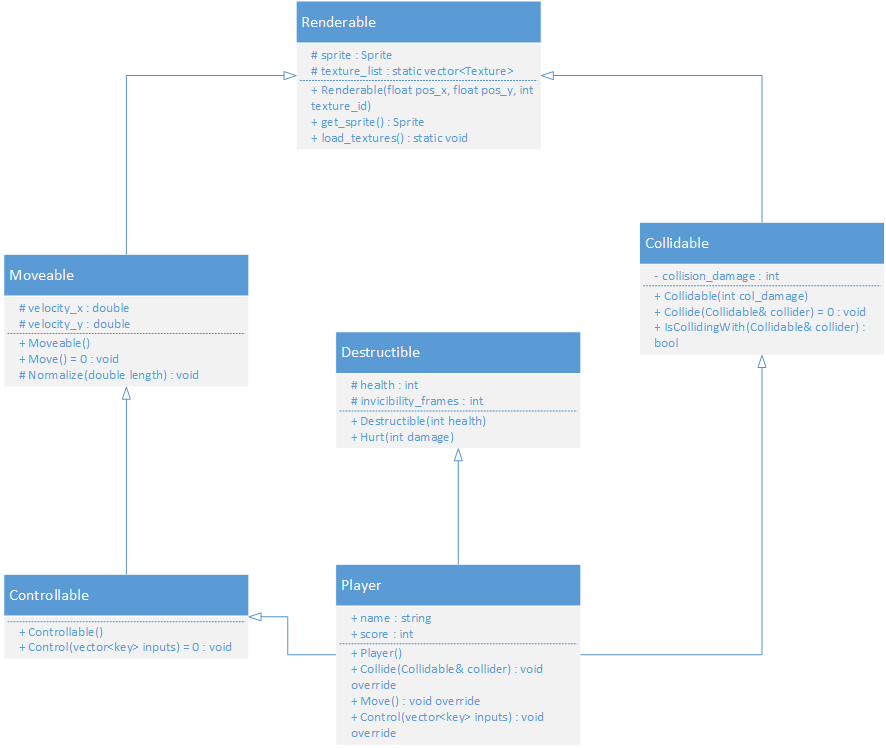
\includegraphics[scale=0.75]{Drawings/player.png}
\end{center}
\clearpage

\subsection{Enemy}
\begin{center}
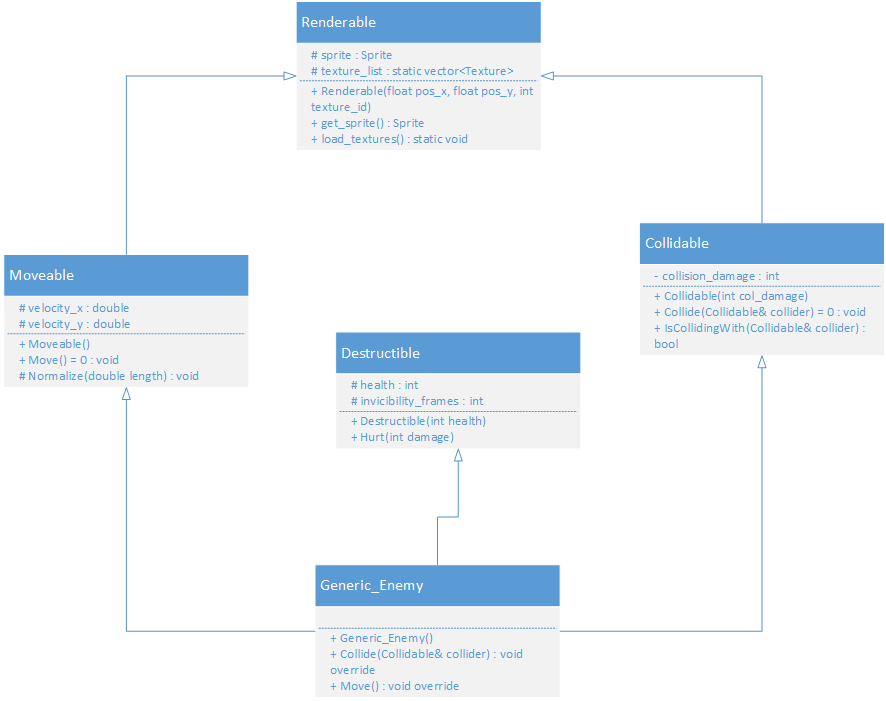
\includegraphics[scale=0.75]{Drawings/enemy.png}
\end{center}
\clearpage

\subsection{Wall}
\begin{center}
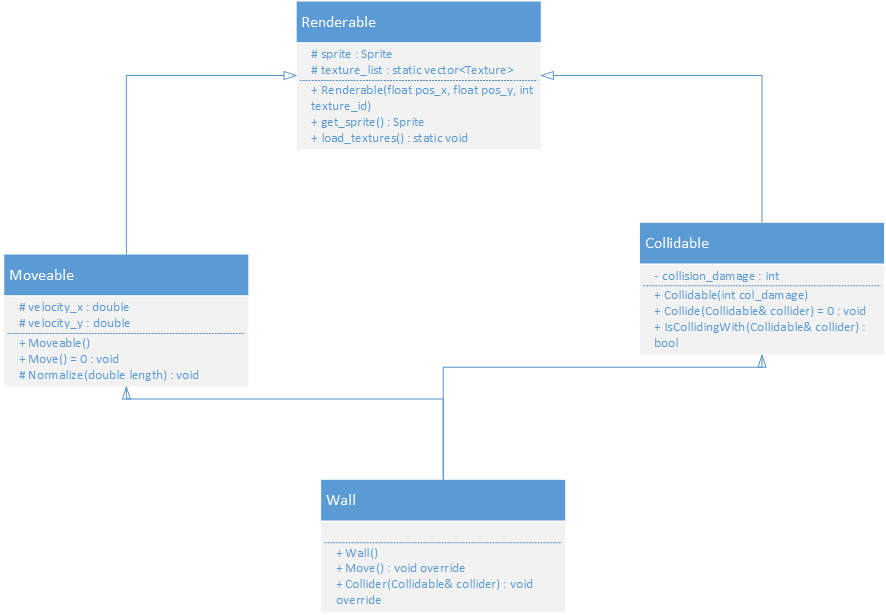
\includegraphics[scale=0.75]{Drawings/wall.png}
\end{center}
\clearpage

\subsection{World}
\begin{center}
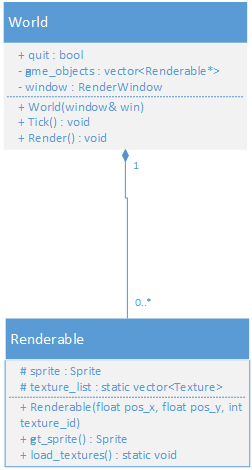
\includegraphics[scale=0.75]{Drawings/world.png}
\end{center}
\clearpage

\section{Detaljbeskrivning}

\subsection{Player}
Spelaren är av klass Player och ärver i något led från klasserna: Controllable,
Destructable, Collidable, Movable \& Renderable.

Player är det objekt spelaren kan kontrollera med hjälp av tangentbord och mus.
Med [W] [A] [S] [D] kan spelaren flytta karaktären på skärmen i X och Y-led,
d.v.s. upp och ned. Med musen kan spelaren sikta, och med vänster musknapp,
skjuta. Kontrollerna fungerar genom Controllable-klassen och rörelserna via
Movable-klassen. Vid rörelse används Collidable-klassen för att detektera
kollisioner, och om en sådan upptäcks tar spelaren skada via
Destructable-klassen och blir sedan odödlig i ett antal bildrutor, angivet i
samma klass. Position av objektet sparas i dess Sprite via Renderable-klassen.
Likaså dess utseende.

Konstruktorn för Renderable är den ända som tar argument. pos\verb|_|x \&
\verb|_| är startpositionerna för objektet. texture\verb|_|id är bilden som
hämtas ur texture\verb|_|list för att representera objektet i världen.

Collide() i Collidable skrivs över för att hantera alla möjliga fall av
kollisioner där collider är det objekt spelaren kolliderade med. (En fiende
till exempel orsakar skada medan en power-up har en slumpässig effekt).

score i spelaren lagrar den nuvarande poängen som samlas med tiden så länge
spelaren överlever.\\

\underline{Player inehåller (utan arv):}

Player()

name : string\\
score : int\\

\underline{Controllable (arv):}

Controllable()\\
Control(vector<key> inputs) : void override\\

\underline{Destructable (arv):}

Destructable()\\
Hurt(int damage)

health : int\\
invincibility\verb|_|frames : int\\

\underline{Collidable (arv):}

Collideable()\\
Collide(Collidable\& collider) : void override\\
isCollidingWith(Collidable\& collider) : bool

colission\verb|_|damage : int\\

\underline{Movable (arv):}

Movable()\\
Move() : void override\\
Normalize(double length) : void

velocity\verb|_|x : double\\
velocity\verb|_|y : double\\

\underline{Renderable (arv):}

Renderable(float pos\verb|_|x, float pos\verb|_|y, int texture\verb|_|id)\\
get\verb|_|sprite() : Sprite\\
load\verb|_|textures() : static void

sprite : Sprite\\
texture\verb|_|list : static vector<Texture>\\


\subsection{World}

World-klassen är till för att ta hand om alla spelobjekt i en gemensam plats.

Tick()-funktionen kallas varje bildruta. Inuti Tick är det tänkt att den går
igenom alla spelobjekt som finns i världen och utför relevanta saker på dem.
Moveable-objekt rör sig ett steg varje Tick(), Collidable-objekt kontrollerar sina
kollisioner och utför lämplig åtgärd på det de kolliderade med.

Tick har även koll på hur lång tid förra bildrutan tog, och applicerar en faktor
t.ex på rörelsemängden av Moveable-objekt. Om en bildruta tog dubbelt så lång tid
att utföra, så rör sig saker dubbelt så mycket mer ruta. Detta ger en konstant
rörelsehastighet på objekt oavsett hur många bilder per sekund som man spelar i.

Render()-funktionen är till för att rita upp alla uppritningsbara (Renderable) objekt
i spelfönstret. World har en referens till ett utanförliggande fönster som den arbetar på.
Render ska loopa igenom alla uppritningsbara spelobjekt, och rita ut de på sina
positioner.

World ska även ha en bool-flagga quit, som håller reda på när spelet ska avslutas.\\

\underline{World inehåller (utan aggregation):}

World()\\
Tick() : void\\
Render() : void

quit : bool\\
game\verb|_|objects : vector<Renderable*>\\
window : RenderWindow\\

\underline{Renderable (aggregation):}

Renderable(float pos\verb|_|x, float pos\verb|_|y, int texture\verb|_|id)\\
get\verb|_|sprite() : Sprite\\
load\verb|_|textures() : static void\\

\clearpage
\section{Designdiskussion}

Designen för spelet är starkt baserat på så kallade "Mix-in klasser". Detta
innebär att man har en klass för varje egenskap som ett objekt ska innehålla,
t.ex att ett objekt är utritningsbart, kan förflytta sig, kan kollidera m.m.

Denna design ska leda till att det är enkelt att utvidga spelet med fler typer
av objekt så som hinder och monster. Man helt enkelt ärver från de egenskaper
man vill att objektet ska ha.

I egenskapsklasserna så har vi en del "pure virtual"-funktioner som är tänkta
att bli överskrivna av underklasser. Till exempel så har Movable-klassen en
funktion Move(), som underklasser kan skriva över, så att flera underklasser
kan ha olika rörelsemönster.

Collidable har en "pure-virtual" Collide()-funktion, där beteende för kollision
med olika klasstyper kan definieras.

En smidig sak är samarbetet mellan egenskapsklasser. De flesta medlemsvariabler
i egenskapsklasser är "protected", vilket innebär att man har tillgång till dem
i underklasser. Detta innebär att om en klass har egenskaperna
Destructible och Collidable, så kan Collide()-funktionen t.ex interagera med
hälsovärdena i Destructible-klassen. Samarbetet bör fungera smidigt mellan alla
egenskapsklasser.

En dålig sida med denna design är att klasser kan bli väldigt sammankopplade.
Om man ändrar på något i Renderable, så kan man kanske behöva ändra på saker i
underklasserna.

En annan dålig sak vi behövde fixa var "diamantproblemet", då en klass ärver
från en basklass två gånger. I detta fall Player som får Renderable-klassen två
gånger. Vi löste detta med Virtual Inheritance, vilket innebär att det endast
får finnas en instans av Renderable i barn-klassen. Detta gjorde konstruktör-
syntaxen i player lite ful.

En alternativ design är att inte ärva Renderable genom de två klasserna, utan
ärva detta separat och istället använde funktioner som tar all information som
tidigare hämtades ur Renderable som argument. Detta hade gjort klasserna mindre
sammankopplade och löst diamantproblemt.



\end{document}
